\chapter{Gameplay}

\section{Menu}
Quando o jogo é iniciando é mostrado um menu.

\begin{figure}[h]
    \centering
    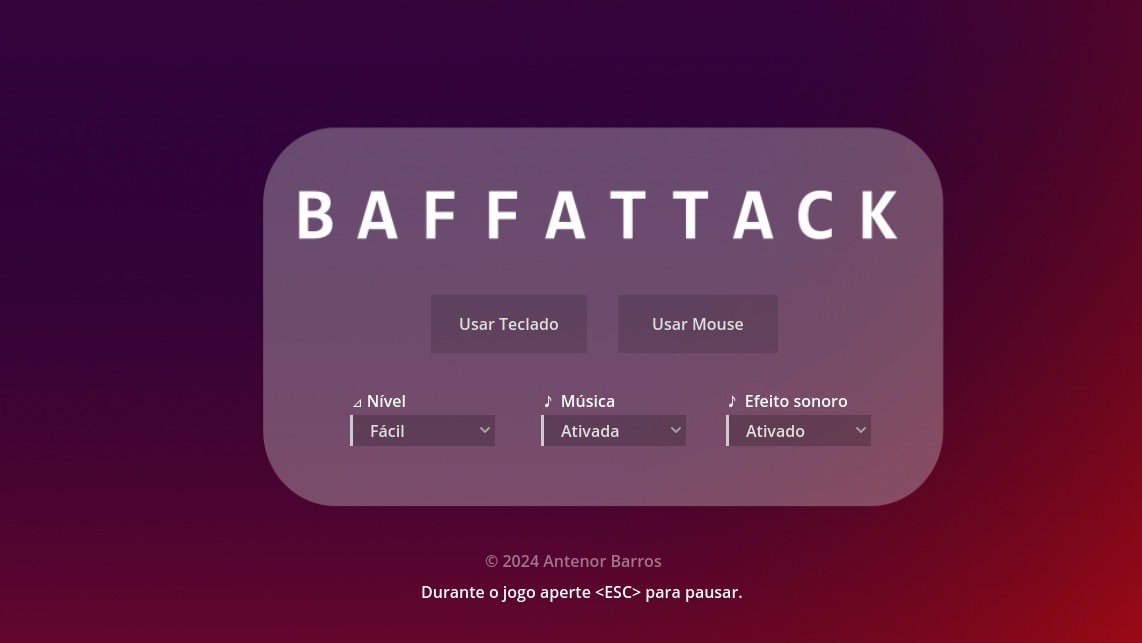
\includegraphics[width=\textwidth]{menu.png}
\end{figure}

Nele é possível escolher o nível de dificuldade, se a música de fundo estará ativa, se os efeitos sonoros estarão ativos e 
qual tipo de controle (teclado ou mouse) será usado.


\begin{figure}[h]
    \centering
    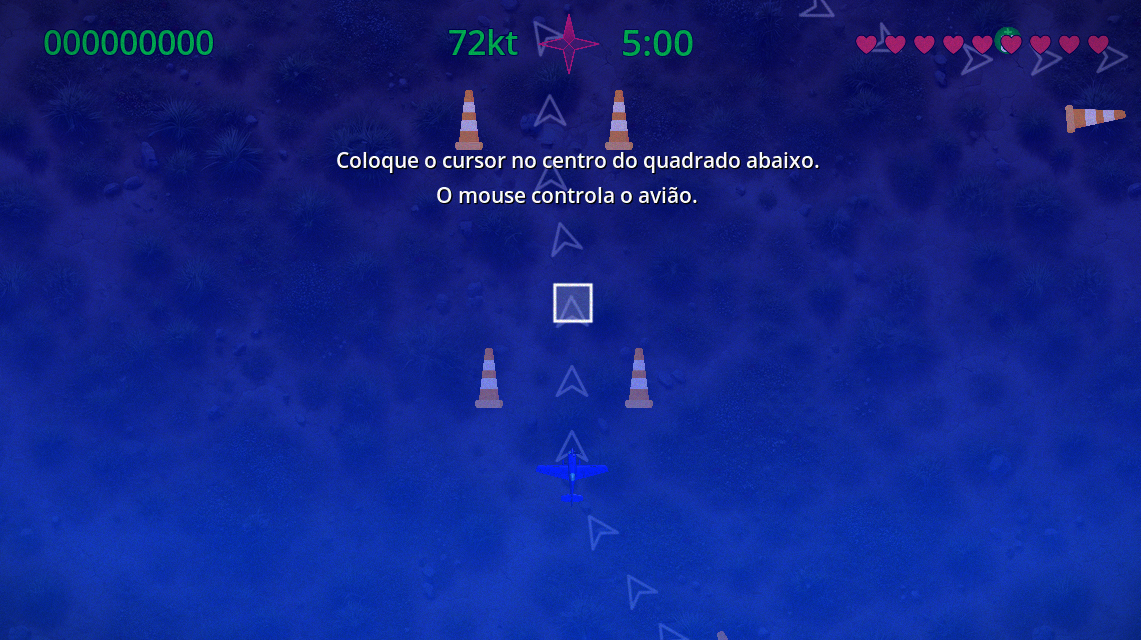
\includegraphics[width=\textwidth]{center.png}
\end{figure}

Na próxima tela o cursor deve ser centralizado no quadrado mostrado para o jogo se inicie.

\section{Jogo}

\begin{figure}[h]
    \centering
    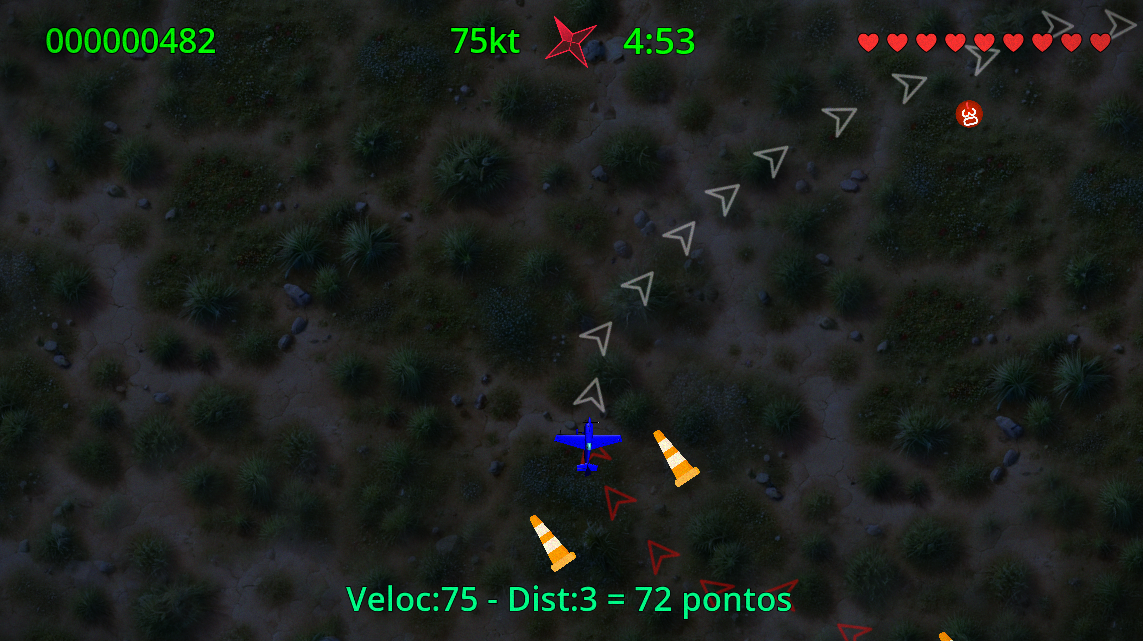
\includegraphics[width=\textwidth]{game.png}
\end{figure}

Na parte de cima do jogo aparece o HUD (head-up display) com as seguintes informações da
esquerda para direita:

\begin{itemize}
\item {Número de pontos}
\item {Velocidade do avião em nós (kt)}
\item {Rosa dos ventos para aumentar a consciência situacional}
\item {Tempo restante}
\item {Ícones de corações representando número de vidas restantes}
\end{itemize}

\chapter{Mecânica}

Como na corrida real, o avião deve passar pelos chamados "Air gates", que são duas colunas (pylon na Red Bull Air Race real) pelas quais a aeronave deve passar no meio, exigindo destreza e timing, já que nenhuma parte do avião pode tocar nas colunas. Na competição real, essas colunas são cones de nylon inflados com ar, como balões que não causam danos à aeronave em caso de colisão, apenas o material se rasga, indicando que o avião não passou corretamente.

\begin{figure}[h]
    \centering
    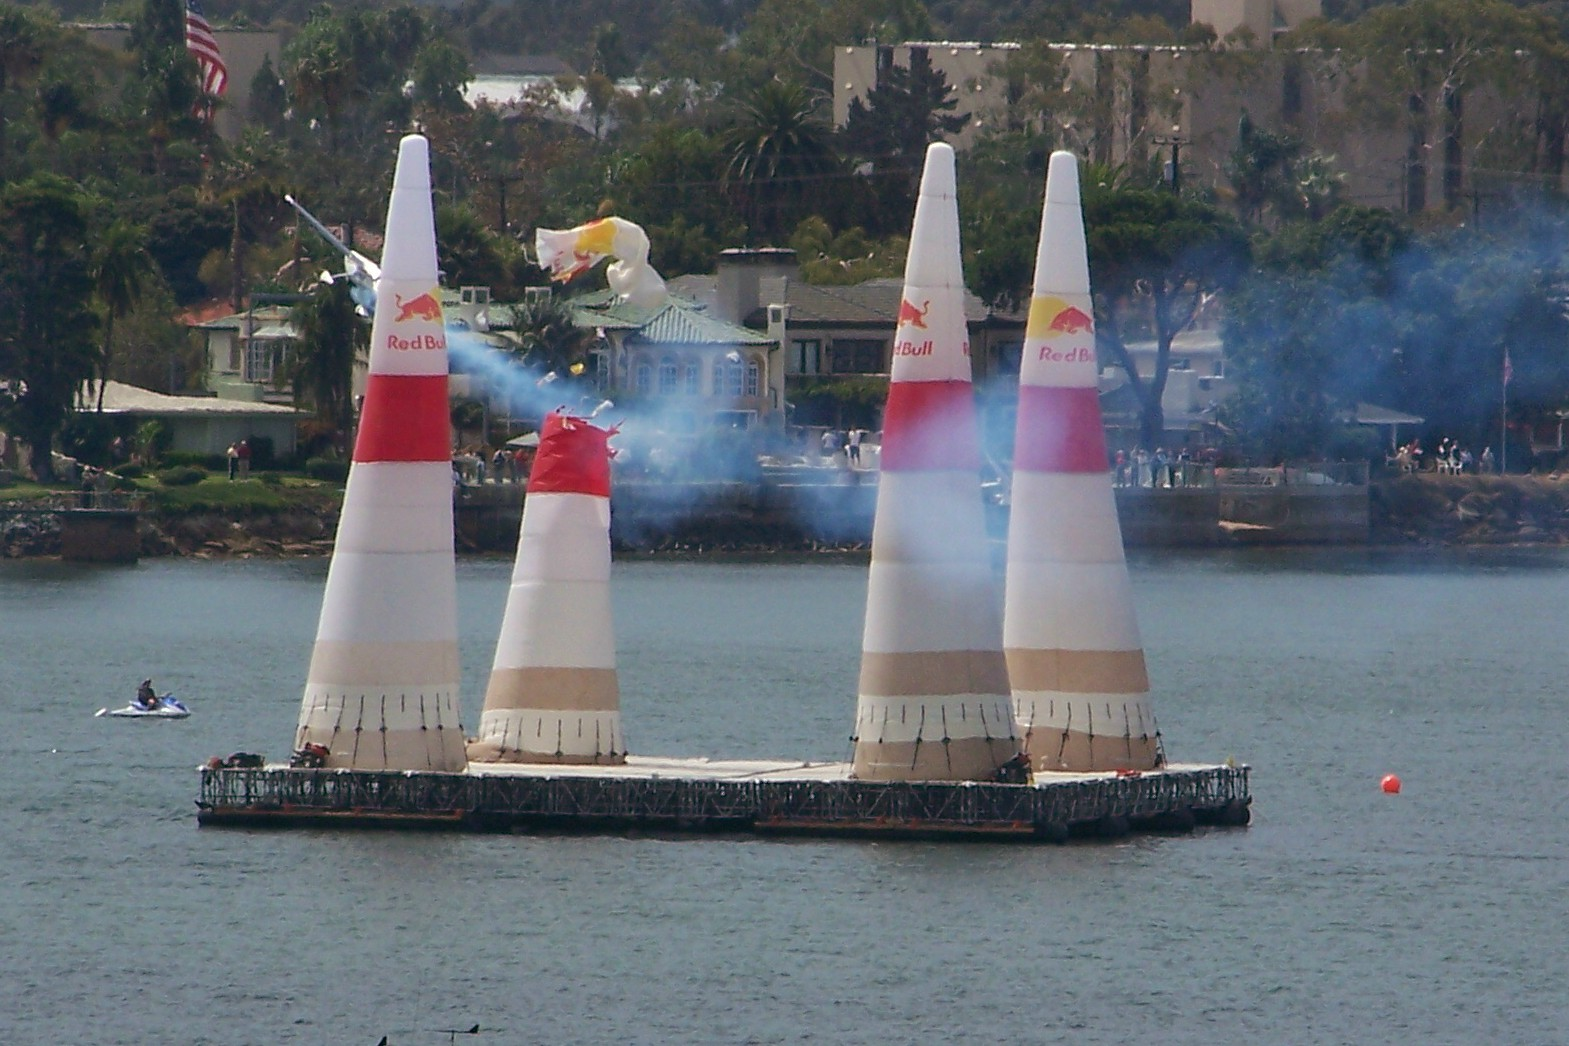
\includegraphics[width=0.8\textwidth]{red-bull-2.jpg}
\end{figure}

\section*{Air Gate}
Existem dois tipos de Air gates: o largo e o estreito.

\subsection*{Largo}
No largo, o avião deve passar sem tocar em nenhuma parte nas colunas. Caso toque, são descontados 100, 200 ou 300 pontos a depender do nível de dificuldade. 
Também são descontadas uma, duas ou três vidas, também, dependendo do nível.

Abaixo, parte do código que trata o evento de colisão
\begin{lstlisting}
private void Explode(Area2D area, String leftOrRight) {
    if (area is Plane)
    {
        hasExplodedJustBefore = true;
        GetNode<Game>("/root/Game").Score -= 100 * Levels.getLevelInfo(Levels.Info.LoseHealthSpeed);
        GetNode<Game>("/root/Game").Health -= Levels.getLevelInfo(Levels.Info.LoseHealthSpeed);
        GetNode<AnimatedSprite2D>("Gate" + leftOrRight + "/Explosion").Visible = true;
        GetNode<AnimatedSprite2D>("Gate" + leftOrRight + "/Explosion").Play();
        GetNode<Godot.Timer>("Gate" + leftOrRight + "/ExplosionTimer").Start();
        GetNode<AudioStreamPlayer>("/root/RootScene/GameScene/Audio/FireSFX").Play();
        var b = GetNode<Banner>("/root/Banner");
        b.showUpperBanner("Atingiu o pylon!", bad: true, "opa você atingiu o pylon", 0.5, 3);
    }
}
\end{lstlisting}

Existe um sentido correto para passar; caso passe no sentido errado, uma, duas ou três vidas são perdidas.

\begin{lstlisting}
if (area is Plane)
    {
        if (lastEnteredFrom == F.Back) 
        {
            lastEnteredFrom = F.None;
            GetNode<Game>("/root/Game").Health -= Levels.getLevelInfo(Levels.Info.LoseHealthSpeed);
            var b = GetNode<Banner>("/root/Banner");
            b.showUpperBanner("Sentido errado!", bad: true);
        }
        else 
        {
            lastEnteredFrom = F.Front;
        }
    }
\end{lstlisting}

\subsection*{Estreito}
No Air gate estreito, as regras anteriores também valem, mas uma dificuldade extra é adicionada. Quando estiver passando, o avião deve estar com as asas inclinadas, mais precisamente com \texttt{abs(R) >= R\_max / 2}. O significado de \texttt{R} e \texttt{R\_max} foi explicado anteriormente. 
Caso esta regra seja descumprida, são descontados 100 pontos e uma vida.

Abaixo o código que verifica a correta inclinação (\texttt{plane.HeadingSpeed})

\begin{lstlisting}
if (lastEnteredFrom == F.Front) 
{
    lastEnteredFrom = F.None;
    if (Math.Abs(plane.HeadingSpeed) > 1.0f)
    {
        float distanceF = GetNode<Path2D>("/root/RootScene/GameScene/AirPath").Curve.GetClosestPoint(area.Position).DistanceSquaredTo(area.Position);
        int distance = (int)Math.Round(distanceF) / 10;
        int speed = GetNode<Game>("/root/Game").Speed;
        int points = 3 * ((int)speed - distance);
        GetNode<Game>("/root/Game").Score += points;
        // GetNode<AudioStreamPlayer>("/root/RootScene/GameScene/Audio/AirGatePassSFX").Play();
        GetNode<Label>("/root/RootScene/GameScene/HUD/AquiredPoints").Text = $"(Veloc:{speed} - Dist:{distance}) x 3 = {points} pontos";
        GetNode<Label>("/root/RootScene/GameScene/HUD/AquiredPoints").Visible = true;
        GetNode<AnimationPlayer>("/root/RootScene/GameScene/HUD/AquiredPoints/AnimationPlayer").Play("AppearAndDisappear");
        GetNode<AudioStreamPlayer>("/root/RootScene/GameScene/Audio/AirGateNarrowPassSFX").Play();
        var b = GetNode<Banner>("/root/Banner");
        b.showUpperBanner("Perfeito!");
    }
    else
    {
        GetNode<Game>("/root/Game").Health -= 1;
        GetNode<Game>("/root/Game").Score -= 100;
        var b = GetNode<Banner>("/root/Banner");
        b.showUpperBanner("Passe com a asa inclinada!", bad: true, AudioName: "passe com a asa inclinada", audioDelay: 0);
        
    }
}
\end{lstlisting}

\section*{Power up/down}
O jogo dura 5 minutos, mas aparecem em posições aleatórias do mapa "power-ups" de tempos que dão 30 segundos extras caso o avião passe por cima de um. 
Este possui a cor verde. Caso esteja na cor vermelha é descontado 30 segundos. Ambos os power-ups desaparecem ao serem passados.

\begin{lstlisting}
public partial class TimePowerDown : TimePowerUp
{
    new private void _on_area_entered(Area2D area)
    {
        if (area is Plane)
        {
            GetNode<Game>("/root/Game").RemainingTime -= 30;
            GetNode<AudioStreamPlayer>("/root/RootScene/GameScene/Audio/LessTime").Play();
            var b = GetNode<Banner>("/root/Banner");
            b.showUpperBanner("Perdeu 30 segundos!", bad: true, AudioName: "perdeu 30 segundos");
            QueueFree();
        }
    }
}
public partial class TimePowerUp : Area2D
{
    public void _on_area_entered(Area2D area)
    {
        if (area is Plane)
        {
            GetNode<Game>("/root/Game").RemainingTime += 30;
            GetNode<AudioStreamPlayer>("/root/RootScene/GameScene/Audio/ExtraTime").Play();
            var b = GetNode<Banner>("/root/Banner");
            b.showUpperBanner("Ganhou 30 segundos!", AudioName: "ganhou 30 segundos");
            QueueFree();
        }
    }
}    
\end{lstlisting}

\section*{ExtraHealth}
Existe também um power up que, caso o avião atravesse-o, é dada uma vida extra.

\begin{lstlisting}
GetNode<Game>("/root/Game").Health += 1;
QueueFree();
var b = GetNode<Banner>("/root/Banner");
b.showUpperBanner("Vida extra!", AudioName: "ganhou vida extra");
GetNode<AudioStreamPlayer>("/root/RootScene/GameScene/Audio/ExtraHealth").Play();
\end{lstlisting}

\section*{Caminho}
O avião deve seguir a ordem de "airgates" mantendo-se dentro de um caminho pre-estabelecido. A cada delta, a distância do avião ao caminho é calculada. A partir de um limiar, o jogador começa a perder ponto em uma razão proporcional à distância do caminho. Caso ele fique muito longe, em poucos segundos seu escore chega a zero e ele perde.

\section*{Término do jogo}
O jogo termina se uma ou mais destas condições ocorrerem:
\begin{enumerate}
    \item O tempo chegar em zero;
    \item Os pontos do jogador ficarem iguais a zero ou negativos.
\end{enumerate}

